\graphicspath{{./img/}} % path to graphics

\section*{\LARGE Введение}
\addcontentsline{toc}{section}{Введение}
Метод системной динамики был изобретен в 1950-х Джеем Форрестером из
Массачусетского Технологического Института (MIT). Используя свой научный и
инженерный опыт, Форрестер искал способ применения законов физики, в
частности, законов электрических цепей, к исследованиям и описанию динамики
процессов социальных и экономических систем.\par
Системная динамика чаще всего используется для разработки долгосрочных
стратегических моделей и предполагает высокий уровень агрегации объектов:
модели системной динамики рассматривают людей, товары, ресурсы и другие
отдельные элементы в количественных терминах.\par
В данной работе будет построенна модель, изучающую распространение
инфекционного заболевания среди населения. Давайте рассмотрим численность
населения, равную 10 000 человек, которую обозначим как TotalPopulation.
Вначале заражен только один человек, а все остальные лишь восприимчивы
к болезни.

\begin{itemize}
	\item Во время болезни один человек в среднем контактирует с другими с
		интенсивностью ContactRateInfectious , равной 1.25 человека в день.
		Если заразившийся человек контактирует с восприимчивым к болезни,
		то вероятность передачи инфекции Infectivity равняется 0.6.
	\item После того, как человек заражается, инкубационный период
		AverageIncubationTime длится 10 дней.
	\item Средняя длительность болезни после инкубационного периода
		AverageIllnessDuration (другими словами, длительность периода, когда
		этот человек может заражать других) составляет 15 дней.
	\item Выздоровевшие люди получают иммунитет к болезни и не могут снова
		заболеть.
\end{itemize}


\clearpage

\section*{\LARGE Выполнение практической работы}
\addcontentsline{toc}{section}{Выполнение практической работы}

\section{Создание диаграммы потоков и накопителей}
Создали новую модель, выбрав пункт меню \textbf{Файл > Создать > Модель}.
Назвали ее SEIR и выберали дни в качестве единиц модельного времени.\par
В данной модели не будет учитываться все разнообразие населения, а лишь
выделины четыре категории людей, имеющие значение для изучаемого нами
процесса:

\begin{itemize}
	\item Susceptible --- Восприимчивые к заражению люди, которые еще не были
		заражены вирусом.
	\item Exposed --- Люди, находящиеся в латентной стадии заражения (они уже
		заражены, но еще не могут заражать других).
	\item Infectious --- Люди в активной стадии заражения (они могут заражать
		других людей).
	\item Recovered --- Выздоровевшие люди (они приобрели иммунитет к
		данному заболеванию).
\end{itemize}

Название модели SEIR --- это аббревиатура, образованная сокращением названий
основных стадий распространения инфекции:
Susceptible -- Exposed -- Infectious -- Recovered.\par
Основная логика модели такова: восприимчивые к заболеванию люди
подвергаются заражению вирусом, болеют и заражают других, а затем
выздоравливают. Чтобы промоделировать перемещение людей между, создали
четырьмя накопителями и добавили три потока.\par
В системной динамике накопители (иногда они также называются уровнями или
фондами) представляют собой переменные, которые эквивалентны объему
определенного «вещества» (это могут быть деньги, знания, люди, жидкости и
т.п).\par
Потоки задают динамику системы. Значения накопителей изменяются с
течением времени именно согласно существующим в системе потокам.
Входящий в накопитель поток увеличивает значение данного накопителя,
исходящий из накопителя поток уменьшает его значение.\par
Далее необходимо создать параметры и зависимости.\par
Связь зависимостей используется для задания зависимости между элементами
диаграммы потоков и накопителей.\par
Итоговая схема модели проиллюстрирована на рисунке~\ref{fig:epidemic:complite}.

\begin{figure}[h!tp]
	\centering
	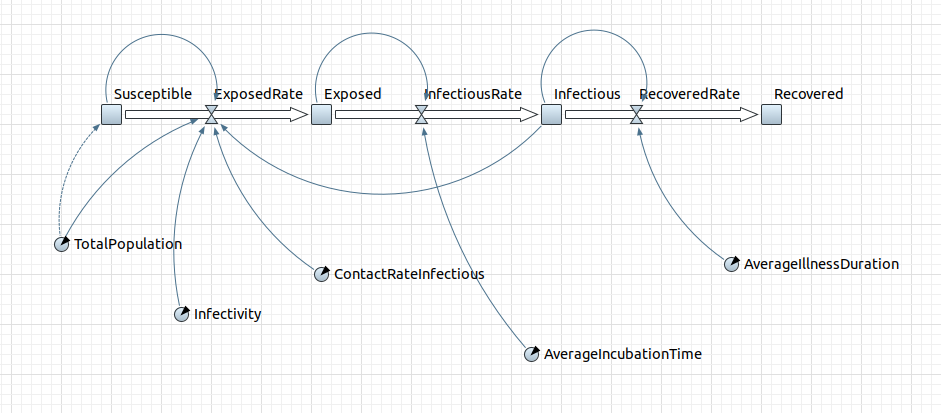
\includegraphics[width=0.9\textwidth]{Screenshot from 2023-03-19 15-39-48}
	\caption{Схема модели распространения эпидемии}
	\label{fig:epidemic:complite}
\end{figure}

Запустив модель и исследовали динамику процесса с помощью похожих на
виджеты информационных окон этих переменных.
Открыть информационное окно переменной можно, щелкнув мышью по этой
переменной (Рисунок~\ref{fig:epidemic:run}).

\begin{figure}[h!tp]
	\centering
	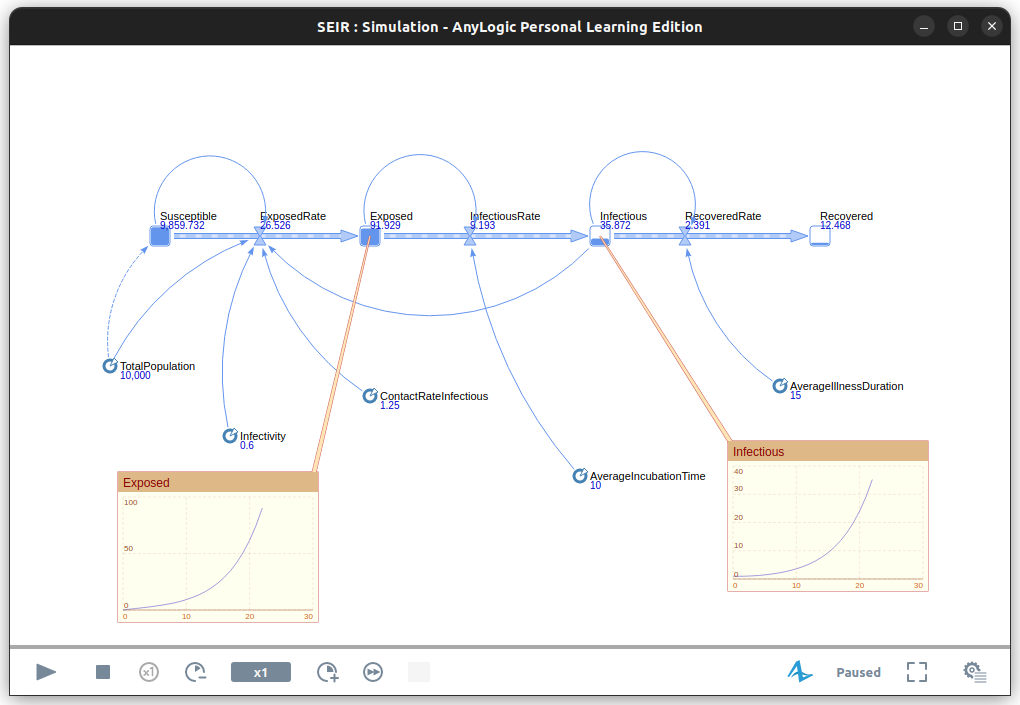
\includegraphics[width=0.9\textwidth]{Screenshot from 2023-03-19 15-46-00}
	\caption{Запуск модели}
	\label{fig:epidemic:run}
\end{figure}

\section{Добавление графика для визуализации динамики процесса}
Системная динамика изучает системы с обратными связями, то есть системы,
образованные (возможно, зависящими друг от друга) циклами обратной связи.
Есть два типа циклов обратной связи: усиливающие и уравновешивающие.
Определить тип цикла можно с помощью следующих правил.
Начните с предположения, что значение переменной увеличивается, и
проследите за изменением значений входящих в цикл переменных.
Цикл является:

\begin{itemize}
	\item \textit{усиливающим}, если после прохождения по циклу видно
		тот же результат, что был допущен при начальном предположении;
	\item \textit{уравновешивающим}, если результат противоречит начальному
		предположению.
\end{itemize}

Есть и другой способ определения типа цикла:

\begin{itemize}
	\item \textit{Усиливающие} циклы содержат четное (или нулевое) количество
		отрицательных связей (то есть, связей, уменьшающих значение
		зависимой переменной).
	\item \textit{Уравновешивающие} циклы содержат нечетное количество
		отрицательных связей.
\end{itemize}

Добавили на диаграмму метку для образовавшегося в системе цикла
зависимостей.\par
Элемент AnyLogic \textbf{Цикл} представляет собой графический значок,
состоящий из метки с описанием смысла цикла и стрелки, показывающей
направление этого цикла. Элемент не задает саму логику зависимостей
в моделируемой системе, а только показывает информацию об образовавшемся
цикле влияний переменных друг на друга.\par
Далее добвили временной график для просмотра динамики изменения
численности каждой категории людей в нашей модели.
Получивщаяся схема проиллюстрирована на рисунке~\ref{fig:epidemic:withGraph}.

\begin{figure}[h!tp]
	\centering
	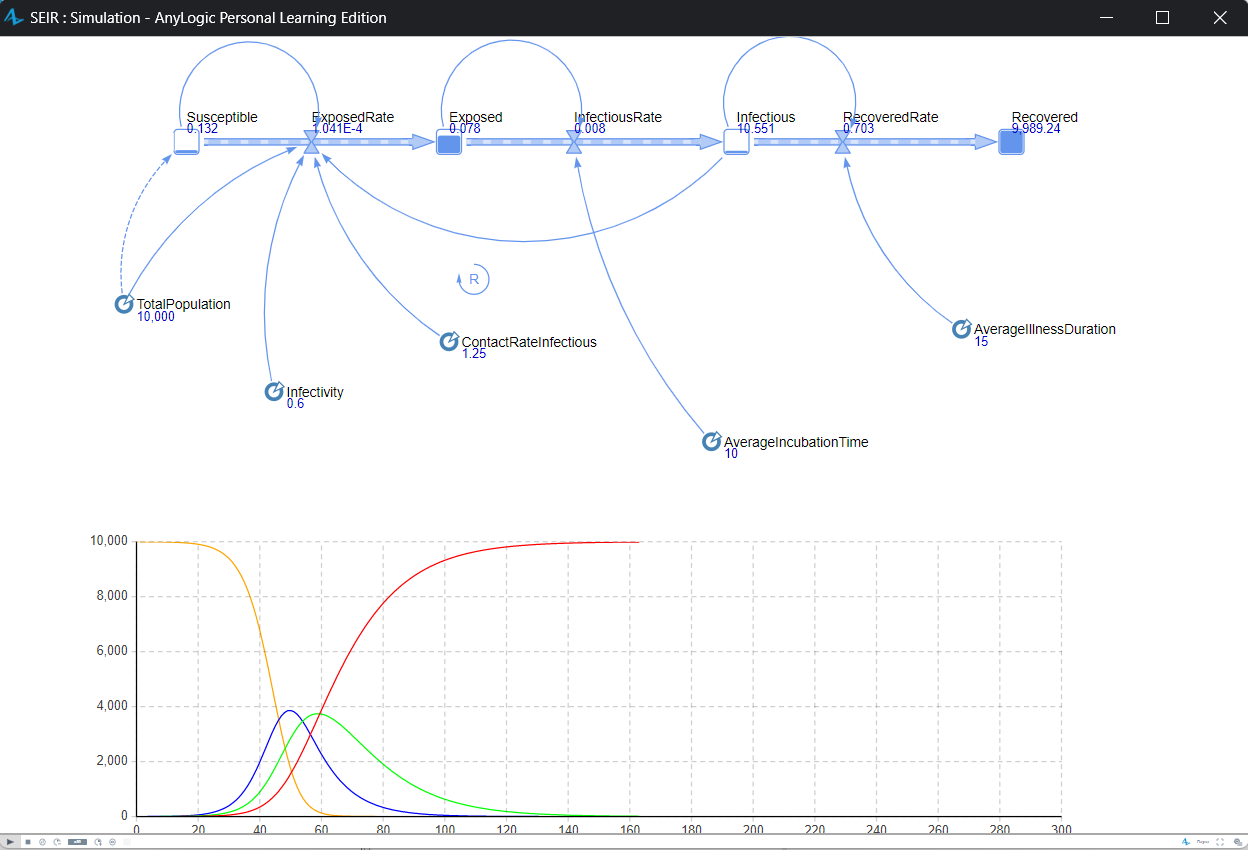
\includegraphics[width=0.9\textwidth]{2023-03-18_17-05-56}
	\caption{Схема модели распространения эпидемии с графиком}
	\label{fig:epidemic:withGraph}
\end{figure}

\section{Эксперимент варьирования параметров}
На этом этапе конструирования модели изучили, как меняется динамика
распространения эпидемии при различных значениях интенсивности контактов
между людьми, воспользовавшись экспериментом варьирования параметров.
Мы запустим этот эксперимент в облачном сервисе («облаке») AnyLogic Cloud.
AnyLogic Cloud --- это облачный сервис, позволяющий запускать модели
онлайн с любого устройства, в том числе с телефонов и планшетов, и
делиться моделями с другими пользователями.\par
Панели \textbf{Входные данные} и \textbf{Выходные данные}, в редакторе
\textbf{Конфигурация запуска}, заполнятся выбранными нами элементами.
Когда модель будет экспортирована в
AnyLogic Cloud, значения выбранных параметров можно будет регулировать.
График будет использоваться для вывода данных облачной модели
(Рисунок~\ref{fig:anlg:confrun}).

\begin{figure}[h!tp]
	\centering
	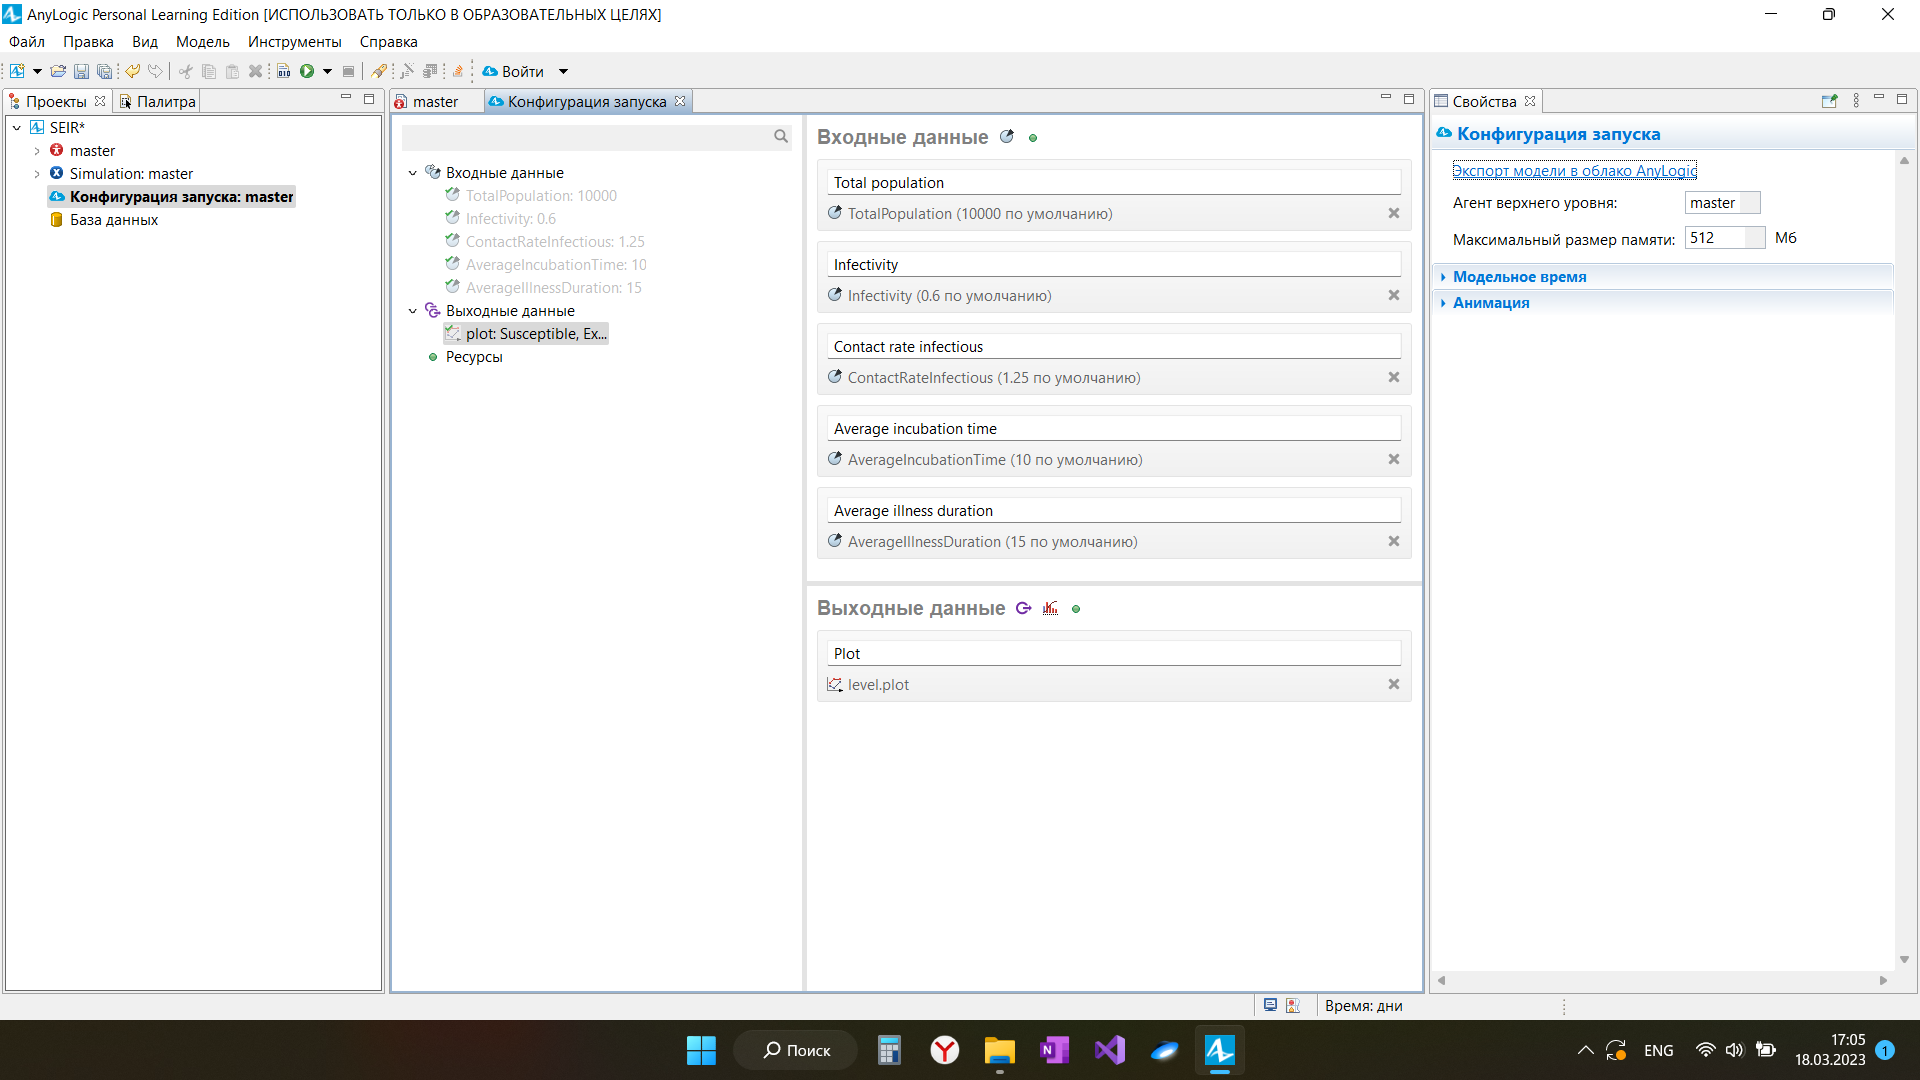
\includegraphics[width=0.9\textwidth]{2023-03-18_17-05-05}
	\caption{Схема модели распространения эпидемии с графиком}
	\label{fig:anlg:confrun}
\end{figure}

Далее, в соответствующем пункте меню, экспортируем модель
в облака AnyLogic.\par
После завершения настройки и загрузки, в новой вкладке установленного по
умолчанию браузера откроется страница AnyLogic Cloud, автоматически
созданная для только что загруженной модели. Обратите внимание --- чтобы
увидеть эту страницу, необходимо предварительно авторизоваться в Cloud.\par
Создали другой эксперимент в Cloud, нажав на кнопку с плюсом
сверху на левой панели. Откроется всплывающее окно New experiment.
В поле Experiment name ввели ContactRateVariation.
И выбрали Variation в выпадающем списке Experiment Type.\par
С помощью \textit{Эксперимента} варьирования параметров можно осуществлять
сложное моделирование, в рамках которого производится серия запусков
модели с отличающимися значениями одного или нескольких параметров.
После завершения эксперимента результаты всех запусков отображаются на
одной диаграмме, что позволяет понять, как изменение значений параметров
влияет на результат прогона модели.\par
Если запустить эксперимент с фиксированными значениями параметров, также
можно оценить влияние случайных факторов на стохастические модели.\par
На левой панели появится еще один эксперимент. В разделе Inputs
отображаются параметры агента верхнего уровня этого эксперимента: в
нашем случае это Main. По умолчанию у всех этих параметров
фиксированные значения, которые не будут изменяться в ходе
моделирования. Чтобы эксперимент варьировал интенсивность
контактов зараженных людей, это поведение нужно настроить в \textbf{Dashboard
editor}.
Нашли параметр \textbf{Contact rate infectious}, измените его тип на
\textbf{Varied in range} в выпадающем списке и сохранили изменения.\par
Указали 0.3 в качестве минимального значения параметра, а 2 --- в качестве
максимального. В поле step введите шаг: 0.1.\par
Затем нажали на кнопку \textbf{Run}, чтобы начать эксперимент варьирования
параметров.\par
Эксперимент варьирования параметров произведет несколько прогонов модели
с отличающимися значениями параметра \textit{Contact rate infectious}
и выведет результаты моделирования на графиках
(Рисунок~\ref{fig:anlg:confrun}).

\begin{figure}[h!tp]
	\centering
	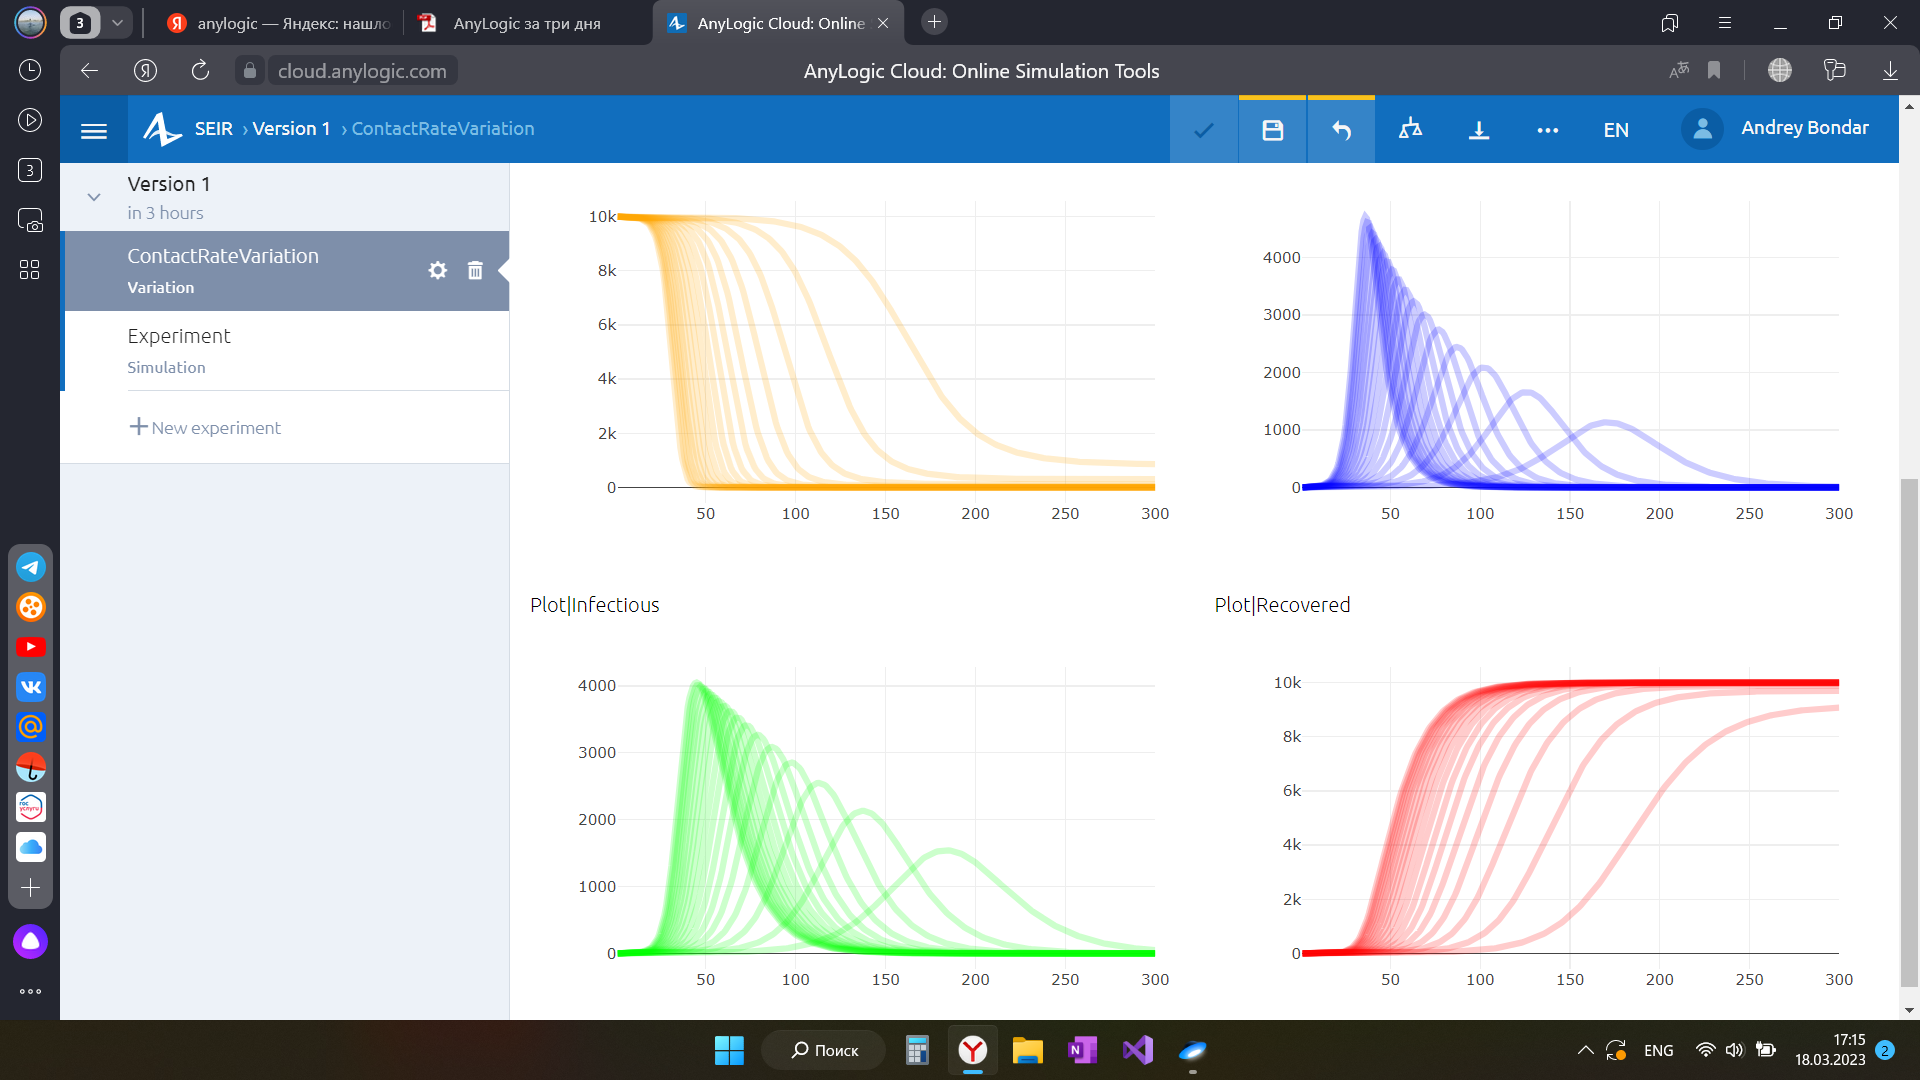
\includegraphics[width=0.9\textwidth]{2023-03-18_17-15-46}
	\caption{Результаты моделирования эксперимента варьирования}
	\label{fig:anlg:confrun}
\end{figure}

Каждый график включает результаты нескольких прогонов (по одной кривой на
запуск) — всего 18. Другими словами, мы видим 18 сценариев заболеваемости
для разных показателей интенсивности контактов, варьирующихся от 0.3 до 2.
Эти сценарии отражают 18 шагов в рамках диапазона значений для параметра,
который мы задали ранее.

\clearpage

\section*{\LARGE Вывод}
\addcontentsline{toc}{section}{Вывод}
В ходе выполнения практической работы научились разрабатывать модели
системной динамики в AnyLogic. А также построили модель распространения
эпидемии, добавлять графики для визуализации динамики процесса и
экспортировать созданную модель в AnyLogic Cloud. И создавать в
AnyLogic Cloud эксперименты с варьированием параметров.

